% region preamble
% mnras_template.tex 
%
% LaTeX template for creating an MNRAS paper
%
% v3.0 released 14 May 2015
% (version numbers match those of mnras.cls)
%
% Copyright (C) Royal Astronomical Society 2015
% Authors:
% Keith T. Smith (Royal Astronomical Society)

% Change log
%
% v3.0 May 2015
%    Renamed to match the new package name
%    Version number matches mnras.cls
%    A few minor tweaks to wording
% v1.0 September 2013
%    Beta testing only - never publicly released
%    First version: a simple (ish) template for creating an MNRAS paper

%%%%%%%%%%%%%%%%%%%%%%%%%%%%%%%%%%%%%%%%%%%%%%%%%%
% Basic setup. Most papers should leave these options alone.
\documentclass[fleqn,usenatbib]{mnras}

% MNRAS is set in Times font. If you don't have this installed (most LaTeX
% installations will be fine) or prefer the old Computer Modern fonts, comment
% out the following line
% Depending on your LaTeX fonts installation, you might get better results with one of these:
%\usepackage{mathptmx}
%\usepackage{txfonts}

% Use vector fonts, so it zooms properly in on-screen viewing software
% Don't change these lines unless you know what you are doing
\usepackage[T1]{fontenc}

% Allow "Thomas van Noord" and "Simon de Laguarde" and alike to be sorted by "N" and "L" etc. in the bibliography.
% Write the name in the bibliography as "\VAN{Noord}{Van}{van} Noord, Thomas"
\DeclareRobustCommand{\VAN}[3]{#2}
\let\VANthebibliography\thebibliography
\def\thebibliography{\DeclareRobustCommand{\VAN}[3]{##3}\VANthebibliography}


%%%%% AUTHORS - PLACE YOUR OWN PACKAGES HERE %%%%%

% Only include extra packages if you really need them. Common packages are:
\usepackage{graphicx}	% Including figure files
\usepackage{amsmath}	% Advanced maths commands
\usepackage{amssymb}	% Extra maths symbols
\usepackage{newtxtext,newtxmath}

%%%%%%%%%%%%%%%%%%%%%%%%%%%%%%%%%%%%%%%%%%%%%%%%%%

\newcommand{\RCR}{\ensuremath{R_{\textrm{CR}}}}
\newcommand{\Rot}{\ensuremath{\mathcal{R}}}
\newcommand{\Vc}{\ensuremath{V_{\textrm{c}} }}
\newcommand{\PS}{\ensuremath{\Omega_{\textrm{p}}}}
\newcommand{\Rb}{\ensuremath{R_{\textrm{b}}}}

\newcommand{\Nbody}{$N$-body}

%%%%% AUTHORS - PLACE YOUR OWN COMMANDS HERE %%%%%

% Please keep new commands to a minimum, and use \newcommand not \def to avoid
% overwriting existing commands. Example:
%\newcommand{\pcm}{\,cm$^{-2}$}	% per cm-squared

% endregion

% region title
%%%%%%%%%%%%%%%%%%% TITLE PAGE %%%%%%%%%%%%%%%%%%%

% Title of the paper, and the short title which is used in the headers.
% Keep the title short and informative.
\title[Stellar Bars and Gas]{Stellar Bars in Isolated Gas-Rich Spiral Galaxies Do Not Slow Down}

\author[A. Beane et al.]{Angus Beane,$^{1}$\thanks{E-mail: angus.beane@cfa.harvard.edu (AB)}
Lars Hernquist,$^{1}$
Elena~D'Onghia,$^{2,3}$
Federico~Marinacci,$^{4}$
Charlie Conroy,$^{1}$
Jia~Qi,$^{5}$\newauthor
Laura~V.~Sales,$^{6}$
Paul~Torrey,$^{5}$
Mark~Vogelsberger$^{7}$
\\
% List of institutions
$^{1}$Center for Astrophysics $|$ Harvard \& Smithsonian,  Cambridge, MA, USA\\
$^{2}$Department of Physics, University of Wisconsin-Madison, Madison, WI, USA\\
$^{3}$Department of Astronomy, University of Wisconsin-Madison, Madison, WI, USA\\
$^{4}$Department of Physics \& Astronomy `Augusto Righi', University of Bologna, Bologna, Italy\\
$^{5}$Department of Astronomy, University of Florida, Gainesville, FL, USA\\
$^{6}$Department of Physics \& Astronomy, University of California, Riverside, CA, USA\\
$^{7}$Department of Physics, Massachusetts Institute of Technology, Cambridge, MA, USA\\
}

% These dates will be filled out by the publisher
\date{Accepted XXX. Received YYY; in original form ZZZ}

% Enter the current year, for the copyright statements etc.
\pubyear{2022}

% endregion

% Don't change these lines
\begin{document}
\label{firstpage}
\pagerange{\pageref{firstpage}--\pageref{lastpage}}
\maketitle

% Abstract of the paper
\begin{abstract}
Elongated bar-like features are ubiquitous in galaxies, occurring at the centers
of approximately two-thirds of spiral disks.  Due to gravitational interactions
between the bar and the other components of galaxies, it is expected that
angular momentum and matter will redistribute over long (Gyr) timescales in
barred galaxies. Previous work ignoring the gas phase of galaxies has
conclusively demonstrated that bars should slow their rotation over time due to
their interaction with dark matter halos. We have performed a simulation of a
Milky Way-like galactic disk hosting a strong bar which includes a
state-of-the-art model of the interstellar medium and a live dark matter halo.
In this simulation the bar pattern does not slow down over time, and instead
remains at a stable, constant rate of rotation. This behavior has been observed
in previous simulations using more simplified models for the interstellar gas
but it has remained unexplained. We propose that the gas phase of the disk and
the dark matter halo act in concert to stabilize the bar pattern speed and
prevent the bar from slowing down or speeding up. We find that in a Milky
Way-like disk, a gas fraction of only about 5\% is necessary for this mechanism
to operate. This result naturally explains why nearly all observed bars rotate
rapidly and is especially relevant for our understanding of how the Milky Way
arrived at its present state.
\end{abstract}

% Select between one and six entries from the list of approved keywords.
% Don't make up new ones.
\begin{keywords}
keyword1 -- keyword2 -- keyword3
\end{keywords}

%%%%%%%%%%%%%%%%%%%%%%%%%%%%%%%%%%%%%%%%%%%%%%%%%%

%%%%%%%%%%%%%%%%% BODY OF PAPER %%%%%%%%%%%%%%%%%%

\section{Introduction}
Elongated bar-like features are ubiquitous in galaxies, occurring at the centers
of approximately two-thirds of spiral disks \citep{2000AJ....119..536E,
2007ApJ...657..790M} and in our own Milky Way \citep{1957AJ.....62...19J,
1991ApJ...379..631B}. The ubiquity of bars is not difficult to explain, since
stellar disks simulated in isolation almost always form bar-like structures
\citep{1971ApJ...168..343H}. Several studies have shown that a spherical
potential, such as from a stellar bulge or dark matter halo, acts to stabilize a
stellar disk against the bar instability \citep{1973ApJ...186..467O,
1976AJ.....81...30H}.

It is more difficult to reconcile numerical simulations with the observed
pattern speeds of extragalactic bars. Currently, the best technique for
measuring the pattern speeds of individual galaxies is the Tremaine-Weinberg
method \citep{1984ApJ...282L...5T, 2011MSAIS..18...23C}. This method has
recently been applied to samples of galaxies from the MaNGA survey
\citep{2019MNRAS.482.1733G, 2020MNRAS.491.3655G}. These recent studies confirm
what was found in earlier studies -- that nearly all extragalactic bars are fast
rotators (i.e., they rotate close to their maximum rotation rate)

This is a problem for theoretical simulations, for which there is ample evidence
that galactic bars should resonantly interact with the dark matter halo, causing
the bar to slow down over time \citep{1992ApJ...400...80H, 2000ApJ...543..704D,
2002MNRAS.330...35A, 2002ApJ...569L..83A, 2003MNRAS.341.1179A,
2003MNRAS.346..251O, 2005MNRAS.363..991H, 2006ApJ...637..214M,
2007MNRAS.375..460W, 2009ApJ...697..293D}. The physical mechanism of this
interaction can be understood as an angular form of dynamical friction between
the bar and the dark matter halo. While studied in detail for the bar
\citep{1984MNRAS.209..729T, 1985MNRAS.213..451W}, this process is generic for
any non-axisymmetric disturbance \citep{1972MNRAS.157....1L}. For an old but
still useful review of bar dynamics, see \citet{1993RPPh...56..173S}

Bar pattern speeds are usually measured using the parameter $\Rot=\RCR/\Rb$,
where \RCR{} is the corotation radius and \Rb{} is the bar length.\footnote{The
radius of corotation \RCR{} is defined for circular orbits as the radius at
which the orbital frequency is equal to the pattern speed, \PS{}, of a given
non-axisymmetric feature. In a galaxy with a constant circular velocity \Vc{},
it is given by $\RCR = \Vc / \PS$.} Galaxies with $\Rot < 1.4$ are considered
``fast rotators'' while galaxies with $\Rot > 1.4$ are considered ``slow
rotators'' \citep{2000ApJ...543..704D}. Galaxies with $\Rot < 1$ are not thought
to be stable \citep{1980AA....81..198C}. Observational estimates of the pattern
speeds of bars indicate that nearly all galaxies have $1 < \Rot <
1.4$ \citep{2011MSAIS..18...23C, 2015AA...576A.102A, 2019MNRAS.482.1733G,
2020MNRAS.491.3655G}.

While the interaction between the bar and a dark matter halo is well-understood
theoretically, this is not the case for the interaction between a bar and a
gaseous disk. Some argue that the gas disk should slow down the bar more, while
others argue that the tendency of the bar to drive gas inwards means the bar
should speed up due to the effect of the gas disk.

In this work, we present a simulation of an isolated, gas-rich disk galaxy. Our
galaxy exhibits some similarities to the Milky Way, described in more detail in
Section XX. Surprisingly, we find that the pattern speed of the bar in this
galaxy is constant with time. We find that with even modest gas fractions of
about 5\%, our isolated galaxy displays no evolution in pattern speed over about
$8\,\textrm{Gyr}$. This behavior has been observed in a few previous works, but
we are the first to exhibit that the behavior ought to be present in a large
fraction of galaxies. We are also the first to provide a physical explanation of
the behavior with clear observational predictions.

In section 2, \dots

% The expectation that a dark matter halo acts to slow down a bar is in conflict
% with observational estimates of bar pattern speeds. Bar rotation rates are
% typically classified by the dimensionless ratio
% % \begin{equation}
% % \Rot = \RCR/R_b\textrm{,}
% % \end{equation}
% where \RCR{} is the radius of corotation and $R_b$ is the length of the
% bar.\footnote{The radius of corotation \RCR{} is defined for circular orbits as
% the radius at which the orbital frequency is equal to the pattern speed,
% $\Omega_p$, of a given non-axisymmetric feature. In a galaxy with a constant
% circular velocity $V_c$, it is given by $\RCR = V_c / \Omega_p$.} Galaxies with
% $\Rot < 1.4$ are considered ``fast rotators'' while galaxies with $\Rot > 1.4$
% are considered ``slow rotators''\cite{2000ApJ...543..704D}. Galaxies with $\Rot
% < 1$ are not thought to be stable\cite{1980AA....81..198C}. Observational
% estimates of the pattern speeds of bars indicate that nearly all galaxies have
% $1 < \Rot < 1.4$\cite{2011MSAIS..18...23C, 2015AA...576A.102A,
% 2019MNRAS.482.1733G, 2020MNRAS.491.3655G}.

% The role of gas on the evolution of the bar is less well-understood. Since the
% gas phase typically only contributes about $10-20\%$ of the mass of a galaxy at
% the present day, one might naively expect it to have a subdominant effect on the
% bar. However, because gas is collisional, it can participate in non-resonant
% angular momentum exchange with the bar\cite{2011MNRAS.415.1027H}. Thus,
% numerical work has shown that the gas phase can have a stronger influence on a
% bar than its contribution to the mass of a galaxy would
% suggest\cite{2010ApJ...719.1470V, 2013MNRAS.429.1949A}.

\section{Methods}

\subsection{Initial Conditions}
The initial setup of the galactic disk used in this work follows closely the
GALAKOS model \citep{2020ApJ...890..117D}, which uses a modified version of the
\texttt{MakeNewDisk} code \citep{2005MNRAS.361..776S}. The GALAKOS model has
three components - a radially exponential and vertically isothermal stellar
disk, and a stellar bulge and dark matter halo following a Hernquist profile
\citep{1990ApJ...356..359H}. All \Nbody{} runs in this work used the same setup
parameters as the GALAKOS disk, more details of which can be found in the
original paper.

The addition of the gas phase was done as follows. The version of
\texttt{MakeNewDisk} used for the original GALAKOS model can generate a gas
disk which is radially exponential and in vertical gravito-hydrodynamic
balance. We modified the radial profile of this code in order to allow us to
generate a disk with a constant surface density within some cut-off radius,
and then exponentially declining beyond that radius with the scale-length of
the stellar disk. Our fiducial model used an initial surface density of
$20\,M_{\odot}/\textrm{pc}^2$ and a cut-off radius of $9.3\,\textrm{kpc}$. The
initial gas disk is generated with a temperature of $10^4\,\textrm{K}$ and
solar metallicity.

After generating the gaseous disk in this way, we stitched the gas disk
together with the GALAKOS \Nbody{} disk (and bulge and dark matter halo) after
the GALAKOS disk has been allowed to evolve for $1.5\,\textrm{Gyr}$. The
purpose of allowing the GALAKOS disk to evolve first for a short period of
time is to allow for the bar to form unimpacted by the presence of the gas
(which would normally disrupt the formation of the bar). Throughout this work,
we consider $t=0$ for the \Nbody{} run to be the time at which we added the
gas phase for the SMUGGLE run (i.e. we ignore the first $1.5\,\textrm{Gyr}$ of
evolution of the \Nbody{} disk when the bar is forming). We made one
additional modification when stitching the gas disk together with the \Nbody{}
disk - we created a hole within the central $4\,\textrm{kpc}$. This hole
guards against an initial dramatic infall of gas within the bar region, which
we found to destroy the bar. It is not uncommon for observed barred galaxies
to have gas deficits in the bar region (though not in the very
center)\cite{1993RPPh...56..173S}, and so our practice of allowing the gas
distribution to have a hole in the central region is consistent with our
choice to begin the simulations with a bar already formed.

\begin{figure}
\centering
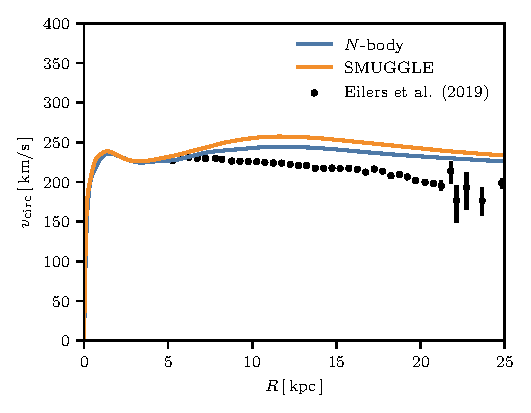
\includegraphics[width=9cm]{fig/vcirc.pdf}
\caption{The circular velocity curve of our initial setups. This
curve is shown for the \Nbody{} run (blue) and the SMUGGLE run (orange)
compared to observational estimates for the Milky
Way \citep{2019ApJ...871..120E}. We see that the circular velocity curve for
both runs is marginally larger than the Milky Way's, but still comparable. The
SMUGGLE circular velocity curve is larger than the \Nbody{} curve due to the
additional mass in the gas phase.}
\label{fig:vcirc}
\end{figure}

Our setup is initially out of equilibrium, but we found that after
$\sim500\,\textrm{Myr}$, the entire system has settled into a steady-state
configuration and initial transients appear not to affect the results after
this point. The constant surface density of the initial gas disk is important
for ensuring the gas disk is dense enough in order for comparisons to real
galaxies to be appropriate.

We computed the circular velocity curve of our model using the \texttt{AGAMA}
package\cite{2019MNRAS.482.1525V}. We fit the baryonic component (stellar
disk, bulge, gas, and newly formed stars) with an axisymmetric cylindrical
spline with $20$ grid points in both the radial and vertical direction
spanning $0.2$ to $50\,\textrm{kpc}$ in the radial direction and from $0.02$
to $10\,\textrm{kpc}$ in the vertical direction. We fit the dark matter halo
using a spherically symmetric multipole fit with a maximum angular harmonic
coefficient of $l=2$. We plot the circular velocity curve in Extended Data
Fig.~\ref{fig:vcirc} compared to observational
estimates\cite{2019ApJ...871..120E}. The SMUGGLE disk (which includes
additional mass in the form of gas) has a slightly higher circular velocity
than the \Nbody{} disk which, itself, is slightly higher than the
observational estimates.

\begin{figure}
    \centering
    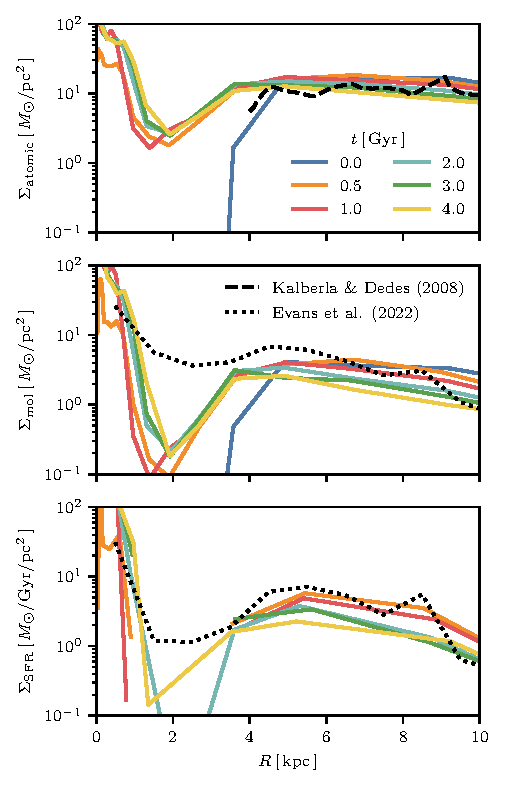
\includegraphics[width=9cm]{fig/surf_dens.pdf}
    \caption{The time evolution of the atomic gas surface density
    (\textit{upper}), molecular gas surface density (\textit{middle}) and the
    star formation rate (SFR) surface density (\textit{lower}) at various times
    during our fiducial simulation. Colored lines indicate the profiles at
    selected times during the simulation while the black dashed lines indicate
    observations for the atomic gas \citep{2008AA...487..951K} and black dotted
    lines indicate a model which allows the CO-to-H$_2$ conversion factor
    $X_{\textrm{CO}}$ to vary with metallicity \citep{2022ApJ...929L..18E}.
    Molecular gas surface densities were provided separately (N. Evans, private
    communication). We see that the molecular gas and SFR surface densities are
    within an order of magnitude of the Milky Way's typical values at all times.
    We see a sharp decrease in the gas and SFR surface densities along the
    extent of the bar from $\sim1$ to $\sim4\,\textrm{kpc}$, related to the gas
    inflow in this region.}
    \label{fig:surf}
\end{figure}

We also show the evolution of the surface density profile in Extended Data
Fig.~\ref{fig:surf} We find that in our simulation the atomic and molecular
gas surface density and the SFR surface density is broadly consistent with the
expected values for the Milky
Way\cite{2008AA...487..951K,2022ApJ...929L..18E}. The discrepancy between $1$
and $4\,\textrm{kpc}$ in the molecular and SFR surface density is likely due
to the fact that the distances to molecular clouds which underlines this work
used a simple kinematic distance based on an axisymmetric model of the Milky
Way\cite{2017ApJ...834...57M}, which is not accurate in the bar region where
gas has large non-circular velocities.

We used a mass resolution of $7.5\times10^3\,M_{\odot}$ for the baryonic
components (initial stellar disk, stellar bulge, and gas) and a mass
resolution of $3.75\times10^4\,M_{\odot}$ for the dark matter halo. This mass
resolution is closest to ``level 3'' in the AURIGA
simulations\cite{2017MNRAS.467..179G}. This corresponds to approximately
$6.4\times10^6$ particles in the stellar disk, $1.1\times10^6$ in the bulge,
$1.2\times10^6$ in the gas disk, and $25.3\times10^6$ in the dark matter halo.
We used a softening length of $0.02\,\textrm{kpc}$ for all components.
Snapshots were saved at equal intervals of $0.005$ in the time units of the
simulation ($\textrm{kpc}/(\textrm{km}/\textrm{s})\sim1\,\textrm{Gyr}$).


% \subsection{Figures and tables}

% Figures and tables should be placed at logical positions in the text. Don't
% worry about the exact layout, which will be handled by the publishers.

% Figures are referred to as e.g. Fig.~\ref{fig:example_figure}, and tables as
% e.g. Table~\ref{tab:example_table}.

% % Example figure
% \begin{figure}
% 	% To include a figure from a file named example.*
% 	% Allowable file formats are eps or ps if compiling using latex
% 	% or pdf, png, jpg if compiling using pdflatex
% 	\includegraphics[width=\columnwidth]{example}
%     \caption{This is an example figure. Captions appear below each figure.
% 	Give enough detail for the reader to understand what they're looking at,
% 	but leave detailed discussion to the main body of the text.}
%     \label{fig:example_figure}
% \end{figure}

% % Example table
% \begin{table}
% 	\centering
% 	\caption{This is an example table. Captions appear above each table.
% 	Remember to define the quantities, symbols and units used.}
% 	\label{tab:example_table}
% 	\begin{tabular}{lccr} % four columns, alignment for each
% 		\hline
% 		A & B & C & D\\
% 		\hline
% 		1 & 2 & 3 & 4\\
% 		2 & 4 & 6 & 8\\
% 		3 & 5 & 7 & 9\\
% 		\hline
% 	\end{tabular}
% \end{table}


\section{Conclusions}

The last numbered section should briefly summarise what has been done, and describe
the final conclusions which the authors draw from their work.

\section*{Acknowledgements}

The Acknowledgements section is not numbered. Here you can thank helpful
colleagues, acknowledge funding agencies, telescopes and facilities used etc.
Try to keep it short.

%%%%%%%%%%%%%%%%%%%%%%%%%%%%%%%%%%%%%%%%%%%%%%%%%%
\section*{Data Availability}

 
The inclusion of a Data Availability Statement is a requirement for articles published in MNRAS. Data Availability Statements provide a standardised format for readers to understand the availability of data underlying the research results described in the article. The statement may refer to original data generated in the course of the study or to third-party data analysed in the article. The statement should describe and provide means of access, where possible, by linking to the data or providing the required accession numbers for the relevant databases or DOIs.




%%%%%%%%%%%%%%%%%%%% REFERENCES %%%%%%%%%%%%%%%%%%

% The best way to enter references is to use BibTeX:

\bibliographystyle{mnras}
\bibliography{ref} % if your bibtex file is called example.bib


% Alternatively you could enter them by hand, like this:
% This method is tedious and prone to error if you have lots of references
%\begin{thebibliography}{99}
%\bibitem[\protect\citeauthoryear{Author}{2012}]{Author2012}
%Author A.~N., 2013, Journal of Improbable Astronomy, 1, 1
%\bibitem[\protect\citeauthoryear{Others}{2013}]{Others2013}
%Others S., 2012, Journal of Interesting Stuff, 17, 198
%\end{thebibliography}

%%%%%%%%%%%%%%%%%%%%%%%%%%%%%%%%%%%%%%%%%%%%%%%%%%

%%%%%%%%%%%%%%%%% APPENDICES %%%%%%%%%%%%%%%%%%%%%

\appendix

\section{Some extra material}

If you want to present additional material which would interrupt the flow of the main paper,
it can be placed in an Appendix which appears after the list of references.

%%%%%%%%%%%%%%%%%%%%%%%%%%%%%%%%%%%%%%%%%%%%%%%%%%


% Don't change these lines
\bsp	% typesetting comment
\label{lastpage}
\end{document}

% End of mnras_template.tex
